\documentclass[12pt,a4paper]{article}

\usepackage[utf8]{inputenc}
\usepackage[T5]{fontenc}
\usepackage[vietnamese]{babel}
\usepackage{amsmath,amssymb}
\usepackage{graphicx}
\usepackage{booktabs}
\usepackage{array}
\usepackage{tabularx}
\usepackage{multirow}
\usepackage{float}
\usepackage{caption}
\usepackage{subcaption}
\usepackage{geometry}
\usepackage{fancyhdr}
\usepackage{hyperref}
\usepackage{xcolor}
\usepackage{enumitem}
\usepackage{listings}
\usepackage[ruled,vlined,linesnumbered]{algorithm2e}

\geometry{left=2.5cm,right=2.5cm,top=2.5cm,bottom=2.5cm,headheight=30pt}

\hypersetup{
    colorlinks=true,
    linkcolor=black,
    urlcolor=blue!70!black,
    citecolor=black
}

\numberwithin{equation}{section}
\numberwithin{table}{section}
\numberwithin{figure}{section}

\captionsetup{
    font=small,
    labelfont=bf,
    labelsep=colon
}

\SetAlgorithmName{Thuật toán}{thuật toán}{Danh sách thuật toán}
\SetKwInput{KwIn}{Đầu vào}
\SetKwInput{KwOut}{Đầu ra}

\pagestyle{fancy}
\fancyhf{}
\fancyhead[R]{%
    \begin{tabular}{r@{\hspace{6pt}}c}
        \texttt{\small Ho Chi Minh City University of Technology} & \multirow{2}{*}{
\includegraphics[height=0.85cm]{figures/hcmut_logo.png}} \\
        \texttt{\small Faculty of Computer Science and Engineering} & \\
    \end{tabular}%
}
\fancyfoot[C]{\thepage}
\renewcommand{\headrulewidth}{0.4pt}
\renewcommand{\footrulewidth}{0pt}

\lstset{
    basicstyle=\ttfamily\small,
    breaklines=true,
    frame=none,
    columns=fullflexible
}

\setlength{\parskip}{4pt}
\setlength{\parindent}{1.2em}

\begin{document}

% ==================== MỤC LỤC ====================
\pagenumbering{roman}
\tableofcontents
\clearpage

\pagenumbering{arabic}
\setcounter{page}{1}
\setcounter{section}{3}

% =========================================================================
% CHƯƠNG 4
% =========================================================================
\section{MÔ HÌNH HÓA VÀ TINH CHỈNH SIÊU THAM SỐ GOM CỤM}

\subsection{Thiết lập thực nghiệm và các chỉ số đánh giá nội bộ}

Đầu vào của giai đoạn mô hình hóa là bảng đặc trưng đã chuẩn hóa \texttt{X\_scaled.csv} từ bước tiền xử lý, gồm $5\,852$ khách hàng và 8 thuộc tính (\texttt{Recency}, \texttt{Frequency}, \texttt{Monetary}, \texttt{AvgOrderValue}, \texttt{UniqueProducts}, \texttt{AvgBasketSize}, \texttt{Tenure} và \texttt{CancelRate}). Ngoài ra, bảng đặc trưng gốc \texttt{customers\_features.csv} cũng được giữ lại để chạy kiểm chứng chéo 5-fold cho K-Means mà không bị rò rỉ dữ liệu. Dữ liệu vẫn giữ nguyên các khách hàng mua sỉ có giá trị giao dịch lớn (ngoại biên) để không làm mất nhóm khách doanh thu cao và để DBSCAN phát hiện ở bước sau.

Các hàm huấn luyện, quét lưới tham số (\texttt{ParameterGrid}), tính chỉ số đánh giá và lưu kết quả được viết tập trung trong \texttt{clustering/models.py} với hạt giống cố định \texttt{RANDOM\_STATE = 42}. Ký hiệu $n = 5\,852$ là tổng số khách hàng, $x_i \in \mathbb{R}^{8}$ là vector đặc trưng của khách hàng thứ $i$, và $k$ là số cụm phân hoạch thành các tập $C_1, \ldots, C_k$. Do bài toán gom cụm không có nhãn mục tiêu, nhóm sử dụng ba chỉ số đánh giá nội bộ phổ biến trong giáo trình~\cite{han2022}:

\begin{itemize}[leftmargin=1.5em]
    \item \textbf{Silhouette Score} ($s \in [-1, 1]$, càng gần $1$ càng tốt): Đo đồng thời độ gắn kết nội cụm và độ tách biệt giữa các cụm. Với mỗi điểm $i$, gọi $a_i$ là khoảng cách trung bình từ $i$ tới các điểm cùng cụm và $b_i$ là khoảng cách trung bình nhỏ nhất từ $i$ tới tất cả các điểm thuộc một cụm khác gần nhất:
    \begin{equation}
        s_i = \frac{b_i - a_i}{\max(a_i, b_i)}.
        \label{eq:silhouette}
    \end{equation}
    Giá trị trung bình toàn tập $\bar{s} = \frac{1}{n}\sum_{i=1}^{n} s_i$ gần $1$ cho thấy cụm gọn và tách rõ; gần $0$ là vùng giáp ranh chồng lấn; giá trị âm ($s_i < 0$) nghĩa là điểm $i$ gần cụm khác hơn cụm đang gán. Với dữ liệu hành vi liên tục 8 chiều, mức $\bar{s}$ khoảng $0,2$ đến $0,3$ là thường gặp nên cần đọc thêm biểu đồ Silhouette chi tiết của từng cụm.

    \item \textbf{Davies--Bouldin Index (DBI)} ($\mathrm{DBI} \ge 0$, càng gần $0$ càng tốt): Đo mức độ chồng lấn trung bình giữa mỗi cụm với cụm gần nó nhất dựa trên tỷ số giữa tổng độ phân tán nội cụm và khoảng cách hai tâm:
    \begin{equation}
        \mathrm{DBI} = \frac{1}{k}\sum_{i=1}^{k} \max_{j \neq i} \left( \frac{\sigma_i + \sigma_j}{\lVert \mu_i - \mu_j \rVert_2} \right),
        \label{eq:dbi}
    \end{equation}
    trong đó $\sigma_i$ là khoảng cách trung bình từ các điểm trong cụm $C_i$ đến tâm $\mu_i$, còn $\lVert \mu_i - \mu_j \rVert_2$ là khoảng cách Euclidean giữa hai tâm cụm $\mu_i$ và $\mu_j$. DBI nhỏ thể hiện cụm có bán kính gọn và các tâm nằm xa nhau; DBI tăng cao đột ngột báo hiệu có cặp cụm bị trộn lẫn.

    \item \textbf{Calinski--Harabasz Index (CHI)} ($\mathrm{CHI} > 0$, càng cao càng tốt): Đo tỷ số giữa phương sai giữa các cụm ($\mathrm{BCSS}$) và phương sai trong cụm ($\mathrm{WCSS}$), chuẩn hóa theo bậc tự do:
    \begin{equation}
        \mathrm{CHI}(k) = \frac{\mathrm{BCSS} / (k - 1)}{\mathrm{WCSS} / (n - k)},
        \label{eq:chi}
    \end{equation}
    với $\mathrm{BCSS} = \sum_{j=1}^{k} |C_j| \lVert \mu_j - \mu \rVert_2^2$ và $\mathrm{WCSS} = \sum_{j=1}^{k} \sum_{x_i \in C_j} \lVert x_i - \mu_j \rVert_2^2$, trong đó $|C_j|$ là số điểm trong cụm $C_j$ và $\mu$ là tâm trung bình của toàn bộ $n$ điểm. CHI lớn nghĩa là các cụm vừa đặc vừa nằm xa nhau. Tuy nhiên trên dữ liệu phân bố liên tục, hệ số chia $(k-1)$ ở tử làm $\mathrm{CHI}(k)$ thường đạt đỉnh tại $k=2$ rồi giảm dần theo $k$. Do đó, CHI không dùng riêng lẻ để chọn $k$ mà dùng để so sánh giữa các thuật toán hoặc kiểu linkage ở cùng một mức $k$.
\end{itemize}

Song song với ba chỉ số trên, bảng tinh chỉnh còn theo dõi kích thước cụm nhỏ nhất và lớn nhất (\texttt{min\_cluster\_size}, \texttt{max\_cluster\_size}) để tránh các cấu hình chỉ tách vài điểm ngoại biên thành một cụm riêng lẻ.

% -------------------------------------------------------------------------
\subsection{Thuật toán K-Means}

\subsubsection{Nguyên lý toán học và mã giả}

K-Means chia $n$ khách hàng $\{x_1, \ldots, x_n\} \subset \mathbb{R}^{8}$ thành $k$ cụm $C_1, \ldots, C_k$ với các tâm $\mu_1, \ldots, \mu_k$ nhằm giảm thiểu tổng bình phương khoảng cách nội cụm (WCSS, hay \texttt{inertia}):
\begin{equation}
    \mathrm{WCSS} = \sum_{j=1}^{k} \sum_{x_i \in C_j} \lVert x_i - \mu_j \rVert_2^2,
    \label{eq:wcss}
\end{equation}
với $\lVert x_i - \mu_j \rVert_2^2$ là bình phương khoảng cách Euclidean từ khách hàng $x_i$ tới tâm cụm $\mu_j$.

Khoảng cách Euclidean được sử dụng vì hai lý do. Thứ nhất, theo toán học, đạo hàm của hàm mục tiêu~(\ref{eq:wcss}) bằng $0$ tại đúng trung bình cộng $\mu_j = \frac{1}{|C_j|}\sum_{x_i \in C_j} x_i$, nên thuật toán Lloyd luôn đảm bảo giảm WCSS sau mỗi bước lặp. Thứ hai, 8 biến đầu vào đều là biến liên tục đã chuẩn hóa về cùng thang đo, và trong bài toán RFM ta quan tâm trực tiếp đến độ lớn chi tiêu hay tần suất mua (khác với Cosine chỉ quan tâm góc và bỏ qua độ lớn giữa 2 vector).

Về mặt hạn chế, do tối ưu tổng bình phương khoảng cách Euclidean và cập nhật tâm bằng trung bình cộng, K-Means nhạy cảm mạnh với chênh lệch thang đo giữa các biến cũng như dữ liệu lệch phải hoặc chứa ngoại biên (các điểm chi tiêu cực lớn có thể kéo lệch tâm cụm). Đây chính là lý do giai đoạn tiền xử lý ở Chương~3 phải áp dụng biến đổi \texttt{log1p} kết hợp \texttt{RobustScaler} trước khi đưa dữ liệu vào mô hình.

Do K-Means nhạy cảm với vị trí khởi tạo tâm ban đầu, nhóm dùng khởi tạo \texttt{k-means++} (chọn tâm sau ưu tiên ở xa các tâm đã chọn theo bình phương khoảng cách) để các tâm phủ đều dữ liệu hơn so với chọn ngẫu nhiên, đồng thời chạy lặp \texttt{n\_init = 10} lần và giữ lại lần có WCSS thấp nhất để tránh cực tiểu cục bộ. Các bước thực hiện được tóm tắt tại Thuật toán~\ref{alg:kmeans}.

\begin{algorithm}[H]
\caption{Thuật toán K-Means (Lloyd kết hợp \texttt{k-means++})}
\label{alg:kmeans}
\KwIn{Tập dữ liệu đã chuẩn hóa $X = \{x_1, \ldots, x_n\}$, số cụm $k$, số lần khởi tạo $R = 10$.}
\KwOut{Tập tâm cụm $\{\mu_1^*, \ldots, \mu_k^*\}$ và nhãn cụm $\{c_1^*, \ldots, c_n^*\}$.}
Đặt $\mathrm{WCSS}_{\min} \leftarrow +\infty$\;
\For{$r = 1, \ldots, R$}{
    Khởi tạo $k$ tâm ban đầu $\{\mu_1, \ldots, \mu_k\}$ bằng phương pháp \texttt{k-means++}\;
    \Repeat{nhãn cụm không đổi hoặc đạt số vòng lặp tối đa}{
        Gán mỗi điểm $x_i$ vào tâm gần nhất: $c_i \leftarrow \arg\min_{1 \le j \le k} \lVert x_i - \mu_j \rVert_2^2$\;
        Cập nhật lại từng tâm cụm: $\mu_j \leftarrow \frac{1}{|C_j|} \sum_{x_i \in C_j} x_i$\;
    }
    Tính $\mathrm{WCSS}_r$ theo Công thức~(\ref{eq:wcss}); nếu $\mathrm{WCSS}_r < \mathrm{WCSS}_{\min}$ thì lưu lại nghiệm hiện tại\;
}
\Return{$\{\mu_1^*, \ldots, \mu_k^*\}, \{c_1^*, \ldots, c_n^*\}$}\;
\end{algorithm}

\subsubsection{Tinh chỉnh số cụm \texorpdfstring{$k$}{k} bằng Elbow và Silhouette}
\label{subsubsec:kmeans_tuning}

Nhóm thử nghiệm $k \in \{2, 3, \ldots, 10\}$ với cấu hình \texttt{init="k-means++"} và \texttt{n\_init=10}. Việc chọn $k$ dựa trên 4 tiêu chí kết hợp:
\begin{enumerate}[leftmargin=1.8em]
    \item \textbf{Elbow Method:} Tìm điểm khuỷu (\texttt{elbow\_k}) nơi WCSS bắt đầu giảm chậm. Notebook ước lượng tự động bằng cách đưa hai trục về cùng thang $[0, 1]$ rồi lấy điểm có khoảng cách lớn nhất dưới dây nối từ $k=2$ đến $k=10$.
    \item \textbf{Bộ ba chỉ số nội bộ:} Đối chiếu Silhouette, Davies--Bouldin và Calinski--Harabasz.
    \item \textbf{Kích thước cụm:} Kiểm tra \texttt{min\_cluster\_size} và \texttt{max\_cluster\_size} để tránh cụm quá nhỏ.
    \item \textbf{Yêu cầu phân khúc:} Đỉnh Silhouette toàn dải thường rơi vào $k=2$, nhưng chia 2 nhóm quá thô cho mục tiêu phân khúc khách hàng phục vụ marketing (đề tài hướng tới khoảng 4 nhóm: VIP, Tiềm năng, Ngủ đông và Cần níu kéo). Vì vậy, notebook ưu tiên chọn $k$ có Silhouette cao nhất trong vùng lân cận điểm khuỷu ($\texttt{elbow\_k} \pm 1$), rồi kiểm tra thêm bằng biểu đồ Silhouette chi tiết.
\end{enumerate}

Kết quả tinh chỉnh trên $k = 2, \ldots, 10$ được ghi nhận trong Bảng~\ref{tab:kmeans_tuning}, kèm đồ thị tại Hình~\ref{fig:kmeans_elbow} và Hình~\ref{fig:kmeans_sil}.

\begin{table}[H]
\centering
\footnotesize
\setlength{\tabcolsep}{6pt}
\resizebox{\textwidth}{!}{%
\begin{tabular}{@{}rrrrrrr@{}}
\toprule
\textbf{$k$} & \textbf{WCSS (Inertia)} & \textbf{Silhouette} & \textbf{DBI} & \textbf{CHI} & \textbf{Min size} & \textbf{Max size} \\
\midrule
2 & 17\,544,64 & 0,2591 & 1,4092 & 2\,512,70 & 2\,795 & 3\,057 \\
3 & 15\,168,35 & 0,1896 & 1,6340 & 1\,911,10 & 1\,398 & 2\,633 \\
\textbf{4*} & \textbf{13\,116,35} & \textbf{0,2177} & \textbf{1,4011} & \textbf{1\,778,08} & \textbf{938} & \textbf{1\,982} \\
5$^\dagger$ & 11\,781,06 & 0,2068 & 1,3655 & 1\,650,14 & 841 & 1\,462 \\
6 & 10\,876,80 & 0,1916 & 1,3609 & 1\,526,82 & 732 & 1\,471 \\
7 & 10\,096,68 & 0,1914 & 1,3515 & 1\,445,70 & 597 & 1\,133 \\
8 & 9\,519,65 & 0,1903 & 1,3600 & 1\,364,65 & 257 & 1\,030 \\
9 & 9\,035,43 & 0,1907 & 1,3841 & 1\,296,99 & 222 & 1\,020 \\
10 & 8\,587,16 & 0,1887 & 1,3836 & 1\,246,74 & 197 & 961 \\
\bottomrule
\end{tabular}}
\caption{Kết quả tinh chỉnh K-Means trên $k = 2, \ldots, 10$ ($^\dagger$điểm khuỷu gợi ý \texttt{elbow\_k = 5}; *mức được chọn \texttt{best\_k = 4}).}
\label{tab:kmeans_tuning}
\end{table}

\begin{figure}[H]
    \centering
    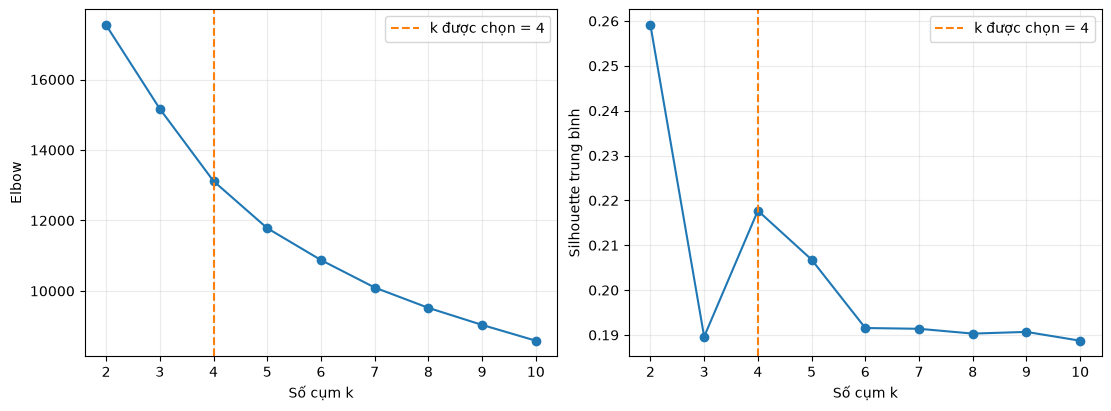
\includegraphics[width=0.90\textwidth]{figures/kmeans_fig1.png}
    \caption{Đường cong Elbow (WCSS) và điểm Silhouette trung bình của K-Means theo số cụm $k$.}
    \label{fig:kmeans_elbow}
\end{figure}

\begin{figure}[H]
    \centering
    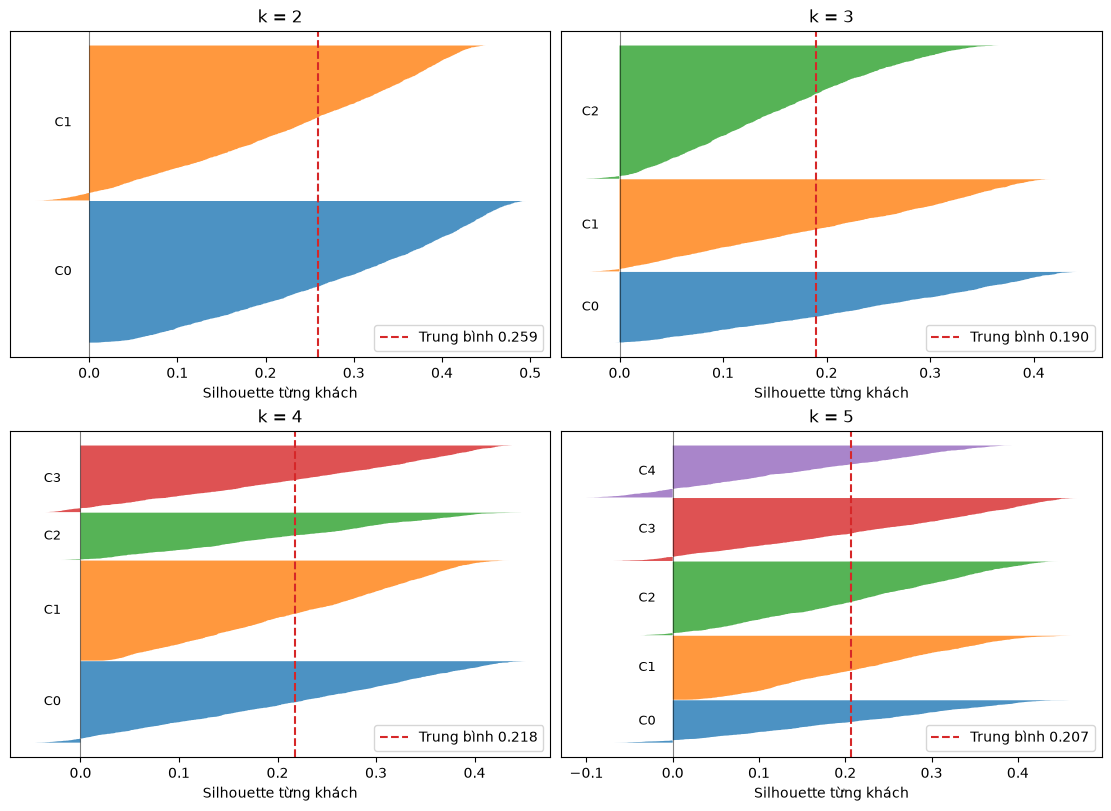
\includegraphics[width=0.84\textwidth]{figures/kmeans_fig2.png}
    \caption{Biểu đồ Silhouette từng khách hàng của K-Means tại $k \in \{2, 3, 4, 5\}$.}
    \label{fig:kmeans_sil}
\end{figure}

Nhận xét từ Bảng~\ref{tab:kmeans_tuning} và hai biểu đồ trên:
\begin{itemize}[leftmargin=1.5em]
    \item Tại $k = 2$, Silhouette cao nhất ($0,2591$) nhưng chỉ tách đôi tập khách hàng ($2\,795$ và $3\,057$ khách), chưa đủ giá trị cho mục đích bài toán là phân khúc khách hàng.
    \item Tại $k = 3$, cả Silhouette ($0,1896$) lẫn Davies--Bouldin ($1,6340$) đều kém hơn rõ rệt so với $k = 2$ và $k = 4$.
    \item Điểm khuỷu tự động gợi ý $\texttt{elbow\_k} = 5$. Xét trong vùng $[4, 6]$, mức $k = 4$ đạt Silhouette cao nhất ($0,2177$), Davies--Bouldin giảm về $1,4011$. Trên Hình~\ref{fig:kmeans_sil}, cả 4 dải cụm đều vượt qua đường trung bình đỏ (đỉnh khoảng $0,44\text{--}0,45$), phần giá trị âm rất ít và kích thước cụm cân đối ($938$; $1\,319$; $1\,613$; $1\,982$ khách).
    \item Sang $k = 5$, Silhouette giảm còn $0,2068$ và xuất hiện cụm có đuôi âm kéo dài tới $-0,10$, cho thấy vùng chồng lấn tăng lên. Vì vậy, nhóm chọn $k = 4$, vừa giữ chất lượng phân cụm tốt vừa khớp với 4 nhóm persona gợi ý của đề tài.
\end{itemize}

\subsubsection{Kiểm tra ngoài mẫu bằng 5-fold Cross-Validation}

Do mô hình K-Means sẽ được đưa lên ứng dụng demo để dự đoán cụm cho khách hàng mới, nhóm thực hiện kiểm chứng 5-fold (\texttt{shuffle=True}, \texttt{random\_state=42}) để đánh giá độ ổn định ngoài mẫu. Trong mỗi lần chia (4 fold train và 1 fold test $T$), phép biến đổi \texttt{log1p} và \texttt{RobustScaler} chỉ được \texttt{fit} trên 4 fold train rồi mới áp dụng sang fold test nhằm tránh rò rỉ dữ liệu. Lỗi gán tâm ngoài mẫu được tính bằng WCSS trung bình trên mỗi khách hàng của fold test:
\begin{equation}
    E_{\mathrm{test}}(k) = \frac{1}{|T|} \sum_{x_i \in T} \min_{1 \le j \le k} \lVert x_i - \hat{\mu}_j \rVert_2^2,
    \label{eq:cv_wcss}
\end{equation}
trong đó $|T|$ là số khách hàng trong fold kiểm tra $T$, còn $\hat{\mu}_1, \ldots, \hat{\mu}_k$ là các tâm cụm học được trên 4 fold huấn luyện.

\begin{table}[H]
\centering
\small
\begin{tabular}{@{}rrrr@{}}
\toprule
\textbf{$k$} & \textbf{\texttt{cv\_test\_wcss\_mean}} & \textbf{\texttt{cv\_test\_wcss\_std}} & \textbf{Mức giảm so với $k-1$} \\
\midrule
2  & 3,0025 & 0,1348 & --- \\
3  & 2,5995 & 0,1087 & $-0,4030$ \\
\textbf{4*} & \textbf{2,2518} & \textbf{0,0896} & $\mathbf{-0,3477}$ \\
5  & 2,0244 & 0,0849 & $-0,2274$ \\
6  & 1,8825 & 0,0774 & $-0,1419$ \\
7  & 1,7389 & 0,0751 & $-0,1436$ \\
8  & 1,6412 & 0,0686 & $-0,0977$ \\
9  & 1,5646 & 0,0606 & $-0,0766$ \\
10 & 1,4799 & 0,0614 & $-0,0847$ \\
\bottomrule
\end{tabular}
\caption{Kết quả lỗi gán tâm ngoài mẫu của K-Means qua 5-fold Cross-Validation (*mức được chọn).}
\label{tab:kmeans_cv}
\end{table}

Từ Bảng~\ref{tab:kmeans_cv} có thể rút ra ba nhận xét củng cố trực tiếp cho lựa chọn $k = 4$:
\begin{itemize}[leftmargin=1.5em]
    \item \textbf{Xu hướng điểm khuỷu giữ nguyên ngoài mẫu:} Từ $k = 2 \to 3$ và $3 \to 4$, lỗi trên fold kiểm tra giảm mạnh khoảng $13,4\%$ mỗi bước ($-0,4030$ và $-0,3477$), cho thấy thêm cụm thứ 4 cải thiện rõ rệt khả năng đại diện cho khách hàng mới. Từ $k = 4 \to 5$ trở đi, mức giảm chậm lại còn $10,1\%$ ($-0,2274$) rồi xuống dưới $0,15$, đồng thuận với vùng điểm khuỷu ở Mục~\ref{subsubsec:kmeans_tuning}.
    \item \textbf{Không có dấu hiệu quá khớp (overfitting):} Tại $k = 4$, WCSS trung bình mỗi khách trên toàn tập huấn luyện ở Bảng~\ref{tab:kmeans_tuning} là $13\,116,35 / 5\,852 = 2,2413$, gần như trùng khớp với lỗi ngoài mẫu trên fold kiểm tra ($2,2518$, chênh lệch dưới $0,5\%$). Điều này cho thấy khi đưa mô hình lên ứng dụng để gán cụm cho khách hàng mới, chất lượng gán tâm hầu như không suy giảm.
    \item \textbf{Độ ổn định cao khi thay đổi dữ liệu:} Độ lệch chuẩn giữa 5 fold tại $k = 4$ là $0,0896$ (khoảng $4,0\%$ so với trung bình $2,2518$, giảm rõ so với $0,1348$ ở $k=2$ và $0,1087$ ở $k=3$). Dù thay đổi $20\%$ tập dữ liệu và \texttt{fit} lại cả \texttt{RobustScaler} lẫn K-Means, 4 tâm cụm vẫn ổn định.
\end{itemize}

\subsubsection{Kiểm tra độ ổn định khởi tạo (ARI) và đối chứng với RFM 3 biến}

Tại $k = 4$, nhóm thử thay đổi cấu hình khởi tạo và đo mức độ tương đồng với mô hình chuẩn bằng chỉ số \textbf{Adjusted Rand Index (ARI)}. Gọi $\mathrm{RI}$ (Rand Index) là tỷ lệ cặp khách hàng được xếp nhất quán (cùng cụm hoặc khác cụm) ở cả hai lần phân cụm, ARI chuẩn hóa $\mathrm{RI}$ bằng cách trừ đi mức trùng hợp ngẫu nhiên kỳ vọng $\mathbb{E}[\mathrm{RI}]$:
\begin{equation}
    \mathrm{ARI} = \frac{\mathrm{RI} - \mathbb{E}[\mathrm{RI}]}{\max(\mathrm{RI}) - \mathbb{E}[\mathrm{RI}]}.
    \label{eq:ari}
\end{equation}
Vì so sánh dựa trên quan hệ từng cặp điểm, ARI không bị ảnh hưởng khi mã số cụm bị đổi thứ tự giữa các lần chạy (ví dụ cụm \texttt{0} đổi thành cụm \texttt{2}); giá trị $\mathrm{ARI} \in [-1, 1]$, trong đó $\mathrm{ARI} = 1$ nghĩa là hai phân hoạch trùng khớp hoàn toàn, $\mathrm{ARI} \approx 0$ tương ứng mức phân cụm ngẫu nhiên.

\begin{table}[H]
\centering
\footnotesize
\resizebox{\textwidth}{!}{%
\begin{tabular}{@{}lrrrl@{}}
\toprule
\textbf{Khởi tạo (\texttt{init})} & \textbf{\texttt{n\_init}} & \textbf{WCSS (Inertia)} & \textbf{ARI vs.\ chuẩn} & \textbf{Ghi chú} \\
\midrule
\texttt{k-means++} & 10 & 13\,116,3474 & 1,0000 & Cấu hình chuẩn (baseline) \\
\texttt{k-means++} & 5  & 13\,116,3474 & 1,0000 & Ra cùng nghiệm \\
\texttt{k-means++} & 20 & 13\,116,3474 & 1,0000 & Không đổi khi tăng số lần khởi tạo \\
\texttt{random}    & 10 & 13\,116,3536 & 0,9988 & Tương đồng 99,88\% \\
\bottomrule
\end{tabular}}
\caption{Kiểm tra độ ổn định của K-Means ($k = 4$) theo các cấu hình khởi tạo.}
\label{tab:kmeans_stability}
\end{table}

Bảng~\ref{tab:kmeans_stability} cho thấy mô hình tại $k = 4$ ít bị ảnh hưởng bởi cách khởi tạo: \texttt{k-means++} với \texttt{n\_init} bằng $5$, $10$ hay $20$ đều hội tụ về cùng một nghiệm ($\mathrm{ARI} = 1,0000$), còn khởi tạo ngẫu nhiên vẫn đạt $\mathrm{ARI} = 0,9988$.

Tiếp theo, để kiểm tra xem 5 biến hành vi bổ sung có cải thiện khả năng tách cụm so với 3 biến RFM cơ bản hay không, nhóm huấn luyện thêm K-Means ($k=4$) trên riêng 3 biến \texttt{Recency}, \texttt{Frequency}, \texttt{Monetary}. Khi so sánh trong Bảng~\ref{tab:rfm_ablation}, ta đọc theo từng cột để giữ nguyên không gian đo khoảng cách (không so chéo giữa cột 3 biến và cột 8 biến vì không gian ít chiều hơn thường cho Silhouette cao hơn).

\begin{table}[H]
\centering
\small
\resizebox{\textwidth}{!}{%
\begin{tabular}{@{}lcc@{}}
\toprule
\textbf{Mô hình K-Means ($k = 4$)} & \textbf{Silhouette trên 3 biến RFM} & \textbf{Silhouette trên 8 biến (RFM + hành vi)} \\
\midrule
RFM thuần túy (3 biến) & \textbf{0,3608} & 0,1215 \\
RFM kết hợp hành vi (8 biến) & 0,1035 & \textbf{0,2177} \\
\bottomrule
\end{tabular}}
\caption{Đối chứng giữa mô hình RFM 3 biến và mô hình mở rộng 8 biến tại $k = 4$.}
\label{tab:rfm_ablation}
\end{table}

Trên không gian 8 biến, mô hình mở rộng đạt Silhouette $0,2177$, cao hơn rõ rệt so với nhãn từ mô hình 3 biến ($0,1215$). Kết quả cho thấy 5 biến hành vi bổ sung mang lại thông tin phân tách mà RFM 3 biến không nắm bắt được. Mô hình K-Means 8 biến ($k = 4$) được lưu ra \texttt{models/kmeans.joblib} và cột \texttt{kmeans} của \texttt{clustering/results/labels.csv}.

% -------------------------------------------------------------------------
\subsection{Thuật toán Gom cụm Phân cấp (Hierarchical Clustering)}

\subsubsection{Nguyên lý, bốn kiểu Linkage và mã giả}

Agglomerative Hierarchical Clustering bắt đầu bằng việc xem mỗi khách hàng là một cụm riêng, rồi lần lượt gộp hai cụm gần nhau nhất cho đến khi toàn bộ dữ liệu gom thành một cây phân cấp (Dendrogram). Khác với K-Means, cây phân cấp là cố định và không có yếu tố ngẫu nhiên. Tuy nhiên, thuật toán cần tính ma trận khoảng cách giữa mọi cặp điểm nên tốn bộ nhớ $O(n^2)$ và thời gian $O(n^2)$ đến $O(n^3)$; với $5\,852$ khách hàng thời gian chạy vẫn chấp nhận được nhưng sẽ chậm nếu dữ liệu lớn hơn nhiều.

Cách đo khoảng cách giữa hai cụm $A$ và $B$ phụ thuộc vào kiểu \textbf{Linkage} (Bảng~\ref{tab:linkage_theory}, với $d(x, y)$ là khoảng cách Euclidean giữa hai điểm $x \in A$ và $y \in B$). Riêng \textbf{Ward linkage} chọn gộp hai cụm sao cho mức tăng tổng bình phương sai số nội cụm là nhỏ nhất (dùng khoảng cách Euclidean):
\begin{equation}
    \Delta(A, B) = \frac{|A|\,|B|}{|A| + |B|} \lVert \mu_A - \mu_B \rVert_2^2,
    \label{eq:ward}
\end{equation}
trong đó $|A|, |B|$ lần lượt là số khách hàng và $\mu_A, \mu_B$ là tâm trung bình của hai cụm $A$ và $B$. Hệ số $\frac{|A|\,|B|}{|A| + |B|}$ lớn hơn khi hai cụm đã đông, nên Ward hạn chế gộp các cụm lớn và có xu hướng chia các cụm đều nhau hơn. Thuật toán được tóm tắt tại Thuật toán~\ref{alg:hierarchical}.

\begin{table}[H]
\centering
\small
\begin{tabularx}{\textwidth}{@{}l>{\raggedright\arraybackslash}p{3.5cm}>{\raggedright\arraybackslash}X>{\raggedright\arraybackslash}X@{}}
\toprule
\textbf{Linkage} & \textbf{Tiêu chí đo $d(A, B)$} & \textbf{Ưu điểm} & \textbf{Nhược điểm} \\
\midrule
\textbf{Single} & $\min_{x\in A, y\in B} d(x,y)$ & Tách được cụm hình dạng kéo dài khi có khoảng trống rõ. & Dễ bị nối chuỗi (\emph{chaining}); hay tách outlier thành cụm 1 điểm. \\
\textbf{Complete} & $\max_{x\in A, y\in B} d(x,y)$ & Tránh nối chuỗi, cụm gọn hơn Single. & Nhạy với outlier vì một điểm xa làm khoảng cách lớn nhất tăng mạnh. \\
\textbf{Average} & $\frac{1}{|A||B|}\sum_{x\in A, y\in B} d(x,y)$ & Trung hòa giữa Single và Complete; giữ khoảng cách gốc khá tốt. & Vẫn hay tách các điểm cực trị ở đuôi thành cụm rất nhỏ. \\
\textbf{Ward} & $\Delta(A,B)$ theo (\ref{eq:ward}) & Tạo cụm gọn, phương sai nội cụm thấp, kích thước cân bằng. & Thiên về cụm dạng cầu; bắt buộc dùng khoảng cách Euclidean. \\
\bottomrule
\end{tabularx}
\caption{So sánh bốn phương pháp Linkage trong Agglomerative Clustering.}
\label{tab:linkage_theory}
\end{table}

\begin{algorithm}[H]
\caption{Thuật toán Agglomerative Hierarchical Clustering}
\label{alg:hierarchical}
\KwIn{Tập dữ liệu $X = \{x_1, \ldots, x_n\}$, phương pháp \texttt{linkage}, số cụm $k$.}
\KwOut{Cây phân cấp $T$ và nhãn cụm tại lát cắt $k$.}
Khởi tạo mỗi điểm là một cụm riêng: $\mathcal{C} \leftarrow \{\{x_1\}, \ldots, \{x_n\}\}$\;
Tính ma trận khoảng cách Euclidean $D(C_a, C_b)$ giữa mọi cặp cụm\;
\While{$|\mathcal{C}| > 1$}{
    Tìm cặp cụm $(A, B) = \arg\min_{C_a \neq C_b} D(C_a, C_b)$ theo tiêu chí \texttt{linkage}\;
    Gộp $C_{\text{mới}} \leftarrow A \cup B$ và lưu bước gộp $(A, B, D(A,B), |C_{\text{mới}}|)$ vào cây $T$\;
    Cập nhật $\mathcal{C} \leftarrow (\mathcal{C} \setminus \{A, B\}) \cup \{C_{\text{mới}}\}$ và tính lại khoảng cách từ $C_{\text{mới}}$ tới các cụm còn lại\;
}
Cắt ngang cây $T$ để thu đúng $k$ cụm\;
\Return{Cây $T$ và nhãn phân cụm}\;
\end{algorithm}

\subsubsection{Thực nghiệm đối chứng bốn kiểu Linkage}

Vì dữ liệu giữ nguyên các khách hàng sỉ (ngoại biên), các linkage dựa trên khoảng cách điểm như \texttt{single}, \texttt{average} và \texttt{complete} có nguy cơ tách vài điểm cực trị thành cụm nhỏ. Để kiểm chứng, nhóm dựng một cây duy nhất cho mỗi linkage bằng hàm \texttt{linkage} (thư viện SciPy), sau đó dùng \texttt{cut\_tree} cắt cùng cây đó tại các mức $k = 2, \ldots, 8$ để tính ba chỉ số nội bộ (Silhouette, Davies--Bouldin, Calinski--Harabasz) cùng kích thước cụm nhỏ nhất và lớn nhất.

Một lát cắt được xem là hợp lệ (không suy biến) khi cụm nhỏ nhất có ít nhất 1\% tổng số khách hàng ($\ge 58$ khách), đồng thời xét riêng nhóm $k \ge 3$ để đủ độ mịn cho mục tiêu phân khúc. Kết quả được tổng hợp ở Bảng~\ref{tab:linkage_summary} và Hình~\ref{fig:hier_compare}.

\begin{table}[H]
\centering
\footnotesize
\resizebox{\textwidth}{!}{%
\begin{tabular}{@{}lccccc@{}}
\toprule
\textbf{Linkage} & \textbf{Hợp lệ ($k \ge 2$)} & \textbf{Hợp lệ ($k \ge 3$)} & \textbf{Min size ($k \ge 3$)} & \textbf{Max size ($k \ge 3$)} & \textbf{Best Silhouette} \\
\midrule
\textbf{ward} & \textbf{7/7} & \textbf{6/6} & \textbf{64} & \textbf{2\,409} & 0,2118 \\
complete      & 1/7 & 0/6 & 5 & 4\,975 & 0,2425 \\
average       & 0/7 & 0/6 & 1 & 5\,845 & \textbf{0,6433} \\
single        & 0/7 & 0/6 & 1 & 5\,850 & 0,5433 \\
\bottomrule
\end{tabular}}
\caption{Tổng hợp kiểm chứng bốn kiểu Linkage trên $5\,852$ khách hàng ($k = 2, \ldots, 8$).}
\label{tab:linkage_summary}
\end{table}

\begin{figure}[H]
    \centering
    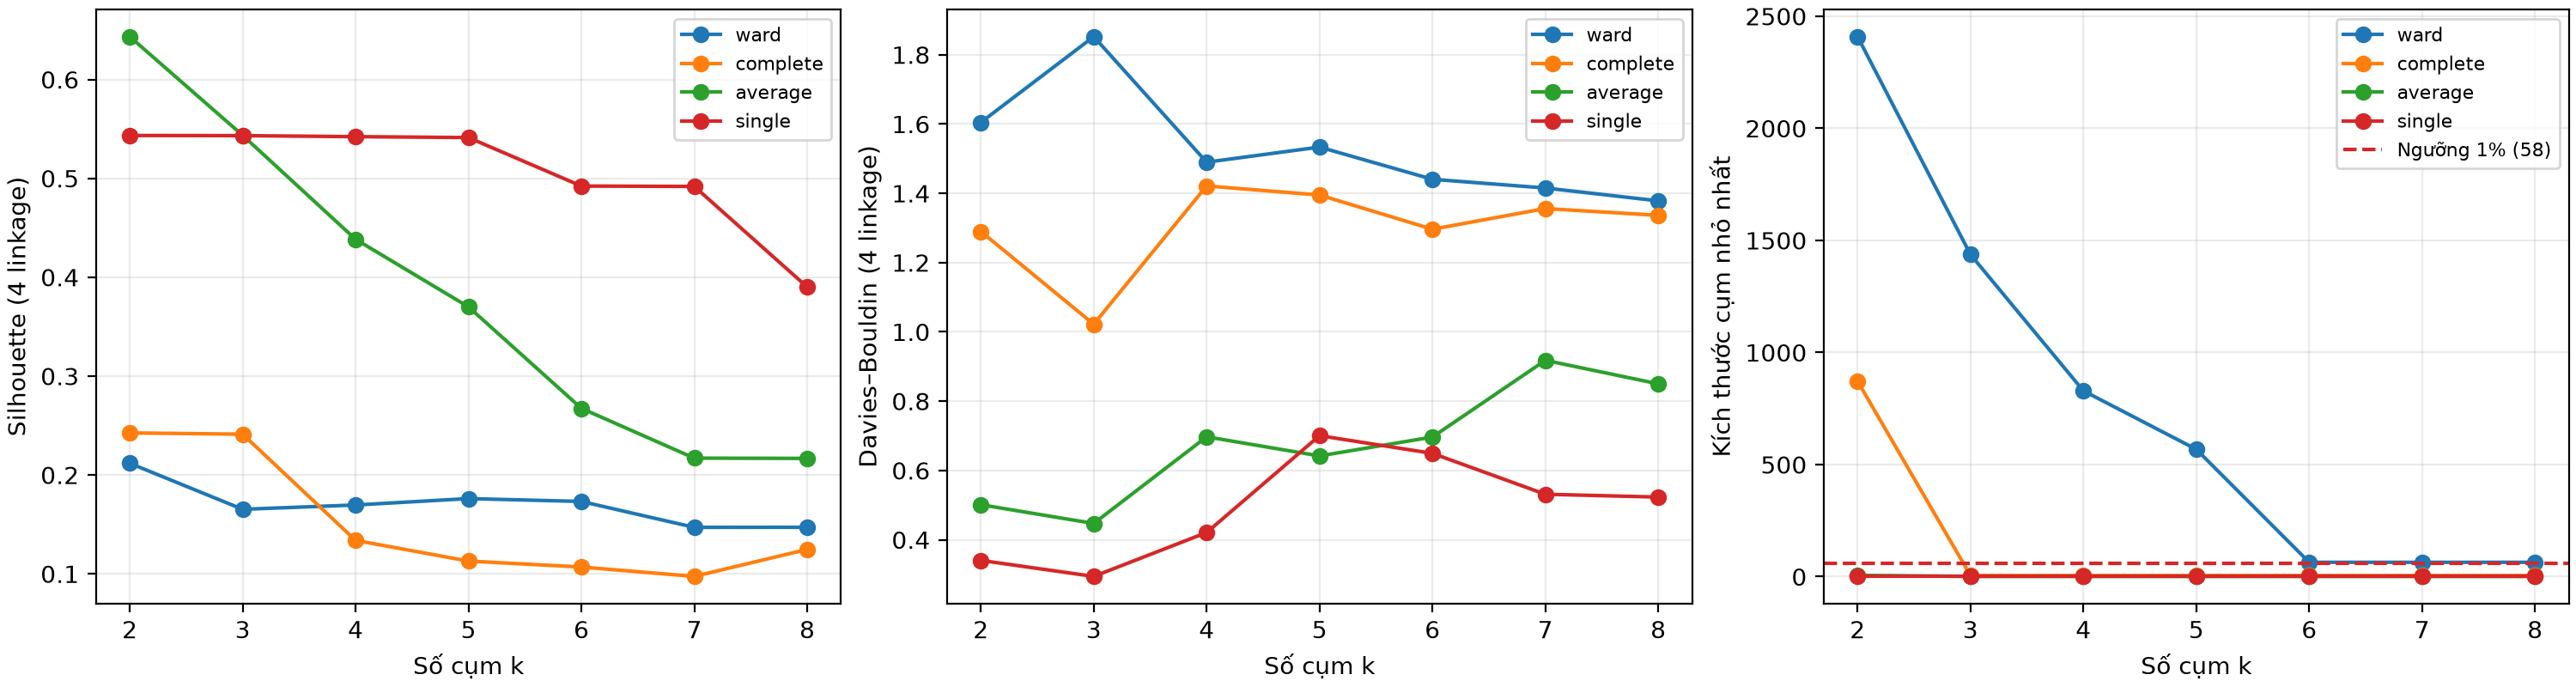
\includegraphics[width=0.95\textwidth]{figures/hierarchical_fig1.png}
    \caption{So sánh 4 kiểu Linkage theo Silhouette, Davies--Bouldin và kích thước cụm nhỏ nhất.}
    \label{fig:hier_compare}
\end{figure}

Bảng~\ref{tab:linkage_summary} cho thấy:
\begin{itemize}[leftmargin=1.5em]
    \item \texttt{average} và \texttt{single} có Silhouette ($0,6433$; $0,5433$) cao nhất nhưng không có lát cắt nào đạt chuẩn ($0/7$): cụm nhỏ nhất chỉ có $1$ khách trong khi có thể lên tới $5\,845\text{--}5\,850$ khách bị gộp vào cùng một cụm (tại $k = 3$). Vì vậy, chỉ nhìn Silhouette mà bỏ qua kích thước cụm sẽ dẫn đến chọn sai mô hình.
    \item \texttt{complete} chỉ qua ngưỡng 1\% tại $k = 2$ (chia lệch $872$ và $4\,980$ khách), còn từ $k \ge 3$ trở đi đều suy biến ($0/6$, cụm nhỏ nhất còn $5$ khách).
    \item Chỉ có \texttt{ward} đạt chuẩn ở tất cả các mức cắt ($7/7$ và $6/6$ ở $k \ge 3$), do đó nhóm chọn \texttt{ward} để tìm số cụm $k$.
\end{itemize}

\subsubsection{Chọn lát cắt trên cây Dendrogram của \texttt{ward}}

Trên ma trận cây \texttt{ward}, tại mức $k$, gọi $h_{\text{lower}}(k)$ là độ cao của lần gộp tạo ra $k$ cụm ($k+1 \to k$) và $h_{\text{upper}}(k)$ là độ cao của lần gộp kế tiếp ($k \to k-1$). Khoảng nhảy dọc và tỷ lệ độ cao được tính bằng:
\begin{equation}
    \Delta h(k) = h_{\text{upper}}(k) - h_{\text{lower}}(k), \qquad r(k) = \frac{h_{\text{upper}}(k)}{h_{\text{lower}}(k)}.
    \label{eq:dendro_gap}
\end{equation}
Khi $\Delta h(k)$ và $r(k)$ lớn, việc gộp từ $k$ xuống $k-1$ cụm làm khoảng cách tăng vọt, cho thấy $k$ nhánh hiện tại khá khác biệt và nên dừng gộp tại đây. Kết quả chi tiết của \texttt{ward} được trình bày trong Bảng~\ref{tab:ward_detail}, Hình~\ref{fig:ward_metrics} và Hình~\ref{fig:ward_dendro}.

\begin{table}[H]
\centering
\footnotesize
\resizebox{\textwidth}{!}{%
\begin{tabular}{@{}rrrrrrrr@{}}
\toprule
\textbf{$k$} & \textbf{Vertical Gap} & \textbf{Height Ratio} & \textbf{Silhouette} & \textbf{DBI} & \textbf{CHI} & \textbf{Min size} & \textbf{Max size} \\
\midrule
2 & 33,94 & 1,450 & 0,2118 & 1,6046 & 1\,834,25 & 2\,409 & 3\,443 \\
3 & 13,50 & 1,218 & 0,1653 & 1,8522 & 1\,590,68 & 1\,437 & 2\,409 \\
4 & 7,96  & 1,147 & 0,1696 & 1,4898 & 1\,463,97 & 829    & 2\,409 \\
\textbf{5*} & \textbf{18,02} & \textbf{1,500} & \textbf{0,1761} & \textbf{1,5334} & \textbf{1\,388,19} & \textbf{568} & \textbf{1\,841} \\
6 & 1,92  & 1,056 & 0,1732 & 1,4404 & 1\,231,36 & 64     & 1\,841 \\
7 & 0,30  & 1,009 & 0,1470 & 1,4153 & 1\,125,89 & 64     & 1\,841 \\
8 & 1,62  & 1,050 & 0,1471 & 1,3782 & 1\,057,77 & 64     & 1\,841 \\
\bottomrule
\end{tabular}}
\caption{Bước nhảy độ cao Dendrogram và chỉ số nội cụm trên nhánh \texttt{ward} (*lát cắt được chọn).}
\label{tab:ward_detail}
\end{table}

\begin{figure}[H]
    \centering
    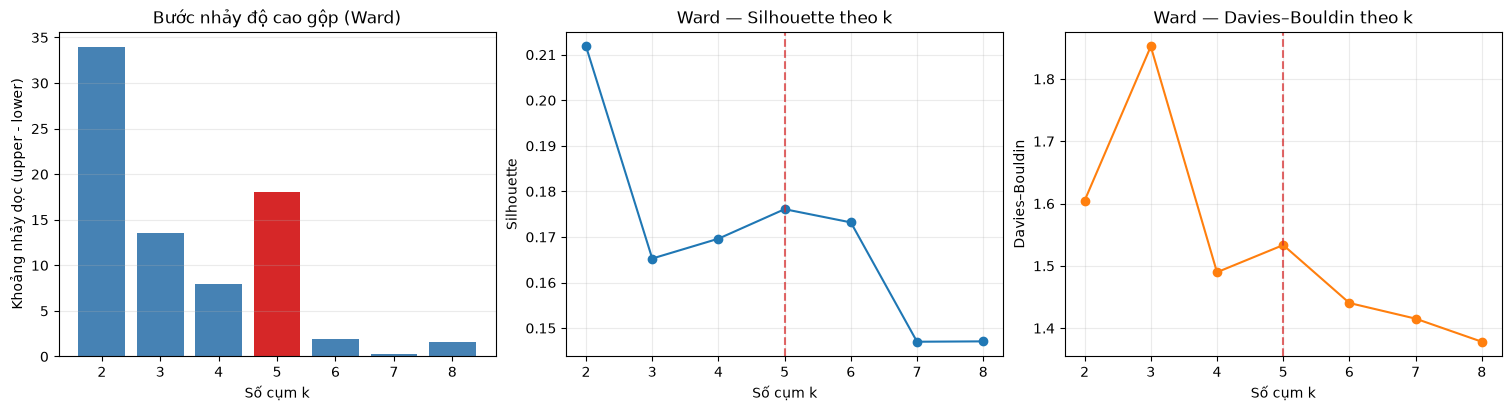
\includegraphics[width=0.95\textwidth]{figures/hierarchical_fig2.png}
    \caption{Bước nhảy độ cao gộp, Silhouette và Davies--Bouldin theo $k$ trên nhánh \texttt{ward}.}
    \label{fig:ward_metrics}
\end{figure}

\begin{figure}[H]
    \centering
    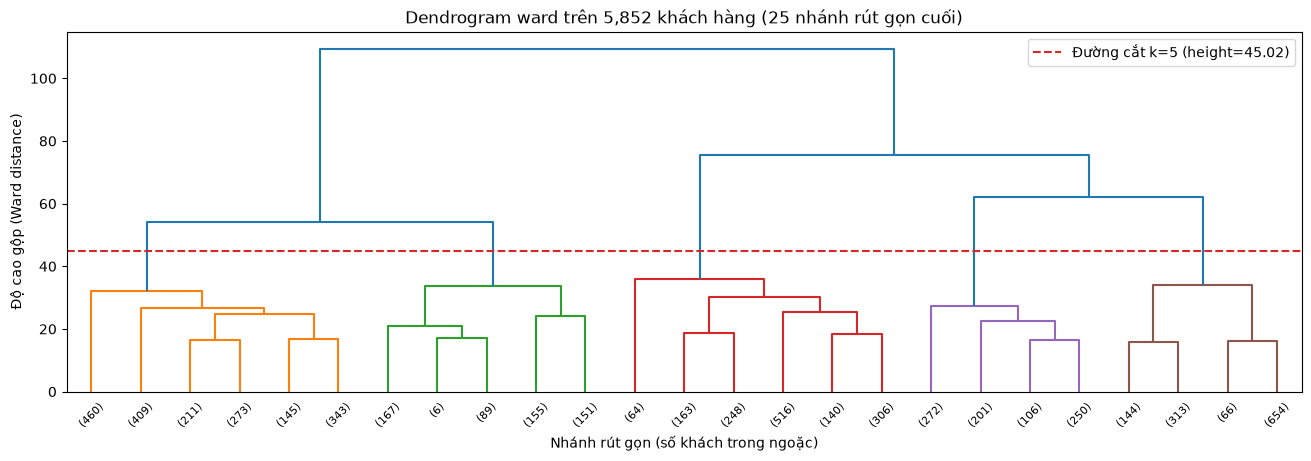
\includegraphics[width=0.94\textwidth]{figures/hierarchical_fig3.png}
    \caption{Dendrogram của \texttt{ward} (25 nhánh rút gọn cuối) với đường cắt ngang tại $k = 5$ ($\text{height} = 45,02$).}
    \label{fig:ward_dendro}
\end{figure}

Xét trong vùng $k \ge 3$, lát cắt \texttt{ward} tại $k = 5$ cho kết quả hợp lý nhất:
\begin{itemize}[leftmargin=1.5em]
    \item Khoảng nhảy dọc đạt $\Delta h = 18,02$ (từ $36,01$ lên $54,03$) với tỷ lệ $r = 1,500\times$, cao nhất trong dải khảo sát $k = 2, \dots, 8$ (lớn hơn cả $1,450\times$ ở $k=2$), tạo ra khoảng trống dọc dễ quan sát trên Hình~\ref{fig:ward_dendro}.
    \item Đạt Silhouette cao nhất trong nhóm $k \ge 3$ ($0,1761$) với 5 cụm có kích thước cân đối ($568$; $829$; $1\,177$; $1\,437$; $1\,841$ khách; cụm nhỏ nhất chiếm $9,7\%$).
    \item Nếu cắt xuống $k = 6$, bước nhảy dọc giảm mạnh xuống còn $1,92$ và cụm nhỏ nhất tụt về $64$ khách ($\approx 1,1\%$). Do đó, lát cắt \texttt{ward, k = 5} được chọn độc lập theo cấu trúc cây và xuất vào cột \texttt{hierarchical} trong \texttt{clustering/results/labels.csv}.
\end{itemize}

% -------------------------------------------------------------------------
\subsection{Thuật toán DBSCAN cho bài toán Phát hiện Ngoại biên}

\subsubsection{Nguyên lý gom cụm theo mật độ và mã giả}

Khác với K-Means và Hierarchical luôn gán mọi khách hàng vào một cụm, DBSCAN gom các điểm nằm trong vùng có mật độ cao và không cần đặt trước số cụm $k$. Trên tập dữ liệu $X$, với bán kính lân cận $\varepsilon$ (\texttt{eps}) và số điểm tối thiểu $m$ (\texttt{min\_samples}), vùng lân cận bán kính $\varepsilon$ của điểm $x$ là tập mọi điểm $y \in X$ cách $x$ không quá $\varepsilon$ theo khoảng cách Euclidean:
\begin{equation}
    N_\varepsilon(x) = \{ y \in X \mid \lVert x - y \rVert_2 \le \varepsilon \}.
    \label{eq:eps_neighborhood}
\end{equation}
Gọi $|N_\varepsilon(x)|$ là số điểm thuộc vùng lân cận trên (tính cả chính $x$), mỗi điểm dữ liệu thuộc một trong ba loại:
\begin{itemize}[leftmargin=1.5em]
    \item \textbf{Điểm lõi (\emph{Core point}):} Thỏa $|N_\varepsilon(x)| \ge m$ (tính cả chính $x$). Các điểm lõi liên thông qua vùng lân cận tạo thành phần lõi của cụm.
    \item \textbf{Điểm biên (\emph{Border point}):} Có $|N_\varepsilon(x)| < m$ nhưng nằm trong vùng lân cận của ít nhất một điểm lõi.
    \item \textbf{Điểm nhiễu / ngoại biên (\emph{Noise}, nhãn \texttt{-1}):} Không phải điểm lõi và cũng không nằm cạnh điểm lõi nào.
\end{itemize}

Do dữ liệu khách hàng phân bố thành một đám mây liên tục và thưa dần ở phần đuôi, mục tiêu khi chạy DBSCAN là tách nhóm khách ngoại biên (nhãn \texttt{-1}) để bộ phận đánh giá kiểm tra hồ sơ giao dịch, chứ không ép ra đúng 4 cụm. Thuật toán được trình bày tại Thuật toán~\ref{alg:dbscan}.

\begin{algorithm}[H]
\caption{Thuật toán DBSCAN}
\label{alg:dbscan}
\KwIn{Tập dữ liệu $X$, bán kính $\varepsilon$, ngưỡng mật độ tối thiểu $m$.}
\KwOut{Nhãn cụm $c_i \in \{-1, 0, 1, \ldots\}$ cho từng điểm $x_i \in X$.}
Đánh dấu mọi điểm trong $X$ là chưa thăm; đặt mã cụm $C \leftarrow -1$\;
\ForEach{điểm $x \in X$ chưa được thăm}{
    Đánh dấu $x$ đã thăm và tìm tập lân cận $N_\varepsilon(x)$ theo~(\ref{eq:eps_neighborhood})\;
    \If{$|N_\varepsilon(x)| < m$}{
        Gán tạm $x$ là nhiễu (\texttt{-1})\;
    }
    \Else{
        Tăng $C \leftarrow C + 1$; gán $x$ vào cụm $C$; khởi tạo hàng đợi $Q \leftarrow N_\varepsilon(x) \setminus \{x\}$\;
        \While{$Q$ khác rỗng}{
            Lấy điểm $y$ ra khỏi $Q$\;
            \If{$y$ đang mang nhãn nhiễu}{Gán lại $y$ vào cụm $C$ (điểm biên)\;}
            \If{$y$ chưa được thăm}{
                Đánh dấu $y$ đã thăm, gán $y$ vào cụm $C$, tìm $N_\varepsilon(y)$\;
                \If{$|N_\varepsilon(y)| \ge m$}{Thêm các điểm trong $N_\varepsilon(y)$ vào $Q$\;}
            }
        }
    }
}
\Return{Nhãn cụm $\{c_1, \ldots, c_n\}$}\;
\end{algorithm}

\subsubsection{Dò bán kính \texorpdfstring{$\varepsilon$}{eps} bằng biểu đồ k-distance}

Trên không gian $d = 8$ chiều, nhóm thử ba mức \texttt{min\_samples} theo các mốc thường dùng: $m = 5$ (mặc định của \texttt{scikit-learn}), $m = d + 1 = 9$ và $m = 2d = 16$ (mật độ chặt hơn cho dữ liệu nhiều chiều). Với mỗi $m$, khoảng cách từ mỗi khách hàng tới láng giềng thứ $m$ (tính cả chính nó) chính là bán kính $\varepsilon$ tối thiểu để điểm đó làm điểm lõi. Khi sắp xếp tăng dần các khoảng cách này, đường cong \emph{k-distance} đi ngang thoai thoải ở vùng đông đúc rồi dốc đứng ở vùng ngoại biên.

Điểm gãy (\emph{knee}) được ước lượng tự động sau khi chuẩn hóa cả hai trục về $[0, 1]$ bằng cách tìm chỉ số $i^*$ có độ võng xa dây nối hai đầu nhất:
\begin{equation}
    i^* = \arg\max_i \left( p_i - \frac{d_{(i)} - d_{(0)}}{d_{\max} - d_{(0)}} \right),
    \label{eq:knee}
\end{equation}
trong đó $d_{(i)}$ là khoảng cách tới láng giềng thứ $m$ của điểm thứ $i$ sau khi sắp xếp tăng dần, $p_i \in [0, 1]$ là thứ hạng chuẩn hóa tương ứng, còn $d_{(0)}$ và $d_{\max}$ lần lượt là giá trị nhỏ nhất và lớn nhất trong $98\%$ phần đầu đường cong. Phần $2\%$ đuôi lớn nhất được tạm bỏ qua trong bước tính biên độ $d_{\max} - d_{(0)}$ để một vài khách mua sỉ quá xa không làm ép dẹt phần đường cong phía trước và kéo lệch điểm gãy. Ba điểm gãy $\varepsilon_{\text{knee}} = d_{(i^*)}$ thu được lần lượt là $0,6684$ ($m=5$), $0,8149$ ($m=9$) và $0,8940$ ($m=16$), thể hiện ở Hình~\ref{fig:dbscan_kdist}.

\begin{figure}[H]
    \centering
    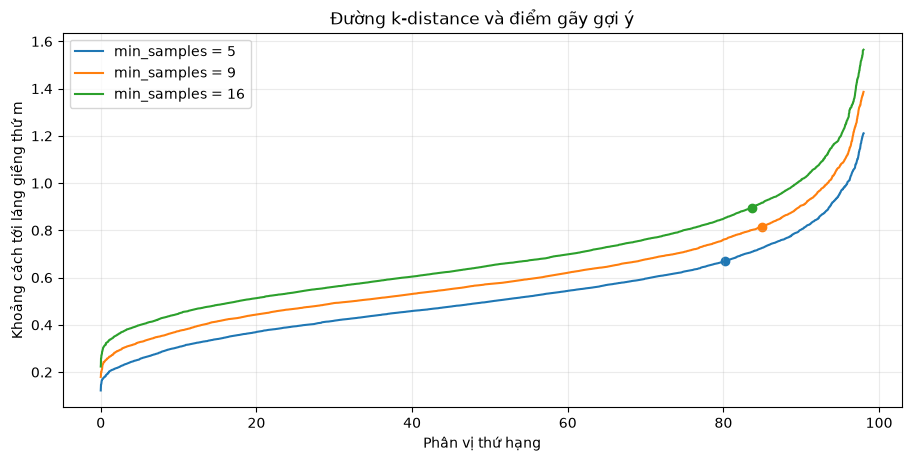
\includegraphics[width=0.82\textwidth]{figures/dbscan_fig1.png}
    \caption{Đường cong k-distance và điểm gãy gợi ý cho ba mức $\texttt{min\_samples} \in \{5, 9, 16\}$.}
    \label{fig:dbscan_kdist}
\end{figure}

\subsubsection{Quét lưới tham số và chọn cấu hình cuối}

Quanh mỗi điểm gãy, nhóm quét 5 hệ số bán kính \texttt{EPS\_FACTORS} gồm $0,85$; $0,90$; $1,00$; $1,10$ và $1,15$ (tổng cộng 15 cấu hình) và tính tỷ lệ nhiễu:
\begin{equation}
    \mathrm{noise\_ratio} = \frac{\#\{i \mid \mathrm{label}_i = -1\}}{n},
    \label{eq:noise_ratio}
\end{equation}
với $\#\{i \mid \mathrm{label}_i = -1\}$ là số khách hàng bị gán nhãn nhiễu \texttt{-1} trên tổng $n$ khách hàng. Toàn bộ diễn biến của 15 cấu hình được trực quan hóa tại Hình~\ref{fig:dbscan_grid} (chi tiết đầy đủ lưu trong \path{clustering/results/tuning_dbscan.csv}).

\begin{figure}[H]
    \centering
    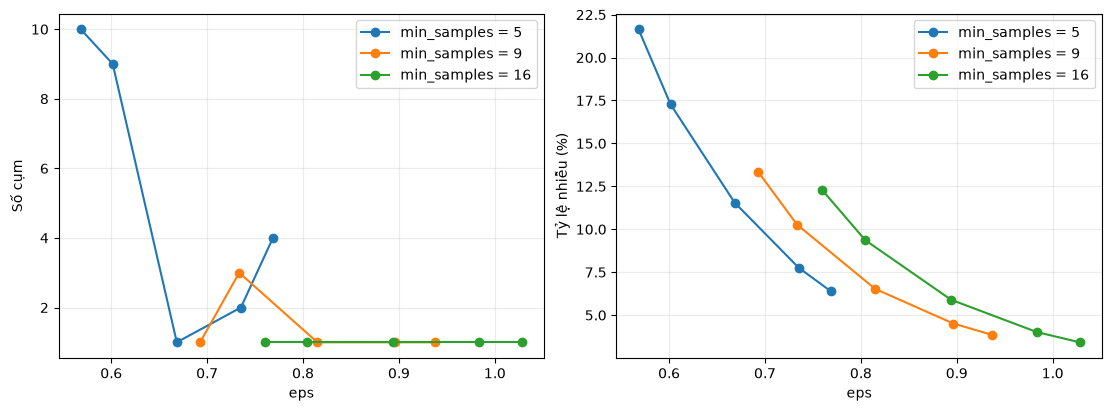
\includegraphics[width=0.88\textwidth]{figures/dbscan_fig2.png}
    \caption{Số cụm và tỷ lệ nhiễu (\%) của DBSCAN trên lưới 15 cấu hình theo bán kính $\varepsilon$ ở ba mức \texttt{min\_samples}.}
    \label{fig:dbscan_grid}
\end{figure}

Tại cả ba điểm gãy ($\text{hệ số } 1,00$), DBSCAN đều cho 1 cụm chính kèm tập nhiễu nên Silhouette không xác định (\texttt{NaN}). Về bán kính, giảm xuống $0,85\text{--}0,90$ đẩy tỷ lệ nhiễu lên cao ($9,4\%\text{--}21,7\%$) và dễ làm vỡ cụm ở $m = 5, 9$, còn tăng lên $1,10\text{--}1,15$ lại nới quá rộng khiến tỷ lệ nhiễu thu hẹp xuống $3,4\%\text{--}7,8\%$ (chỉ còn $3,4\%\text{--}4,5\%$ ở $m = 9$ và $m = 16$); do đó, các điểm gãy ($\text{hệ số } 1,00$) được lấy làm ba ứng viên chính. Ba ứng viên này được xếp hạng theo thứ tự ba tiêu chí:
\begin{enumerate}[leftmargin=1.8em]
    \item \textbf{Ổn định số cụm (\texttt{cluster\_stable}):} Số cụm giữ nguyên khi dịch bán kính $\pm 10\%$ quanh điểm gãy ($0,90\varepsilon_{\text{knee}} \to 1,00\varepsilon_{\text{knee}} \to 1,10\varepsilon_{\text{knee}}$), tránh cấu hình nhạy cảm dễ tách cụm nhỏ giả tạo.
    \item \textbf{Tỷ lệ nhiễu hợp lý (\texttt{noise\_in\_1\_10\_pct}):} Tỷ lệ ngoại biên nằm trong khoảng $1\%\text{--}10\%$, đủ lọc nhóm bất thường mà không gán nhầm quá nhiều khách hàng phổ thông.
    \item \textbf{Độ ổn định tập nhiễu (\texttt{noise\_overlap}):} Khi giữ cố định $m$ và tăng $\varepsilon$, tập nhiễu chỉ thu hẹp ($\mathrm{Noise}_{1,10} \subseteq \mathrm{Noise}_{0,90}$), nên độ chồng lấp Jaccard giữa hai mức $\pm 10\%$ rút gọn thành:
    \begin{equation}
        \mathrm{noise\_overlap}(m) = \frac{|\mathrm{Noise}_{1,10}|}{|\mathrm{Noise}_{0,90}|},
        \label{eq:noise_overlap}
    \end{equation}
    trong đó $|\mathrm{Noise}_{1,10}|$ và $|\mathrm{Noise}_{0,90}|$ lần lượt là số điểm nhiễu tại bán kính $1,10\,\varepsilon_{\text{knee}}$ và $0,90\,\varepsilon_{\text{knee}}$ (tỷ số càng cao tập ngoại biên càng ít biến động).
\end{enumerate}

\begin{table}[H]
\centering
\footnotesize
\resizebox{\textwidth}{!}{%
\begin{tabular}{@{}rrcrcrc@{}}
\toprule
\textbf{\texttt{min\_samples}} & \textbf{$\varepsilon_{\text{knee}}$} & \textbf{Số cụm ($0,90 \to 1,00 \to 1,10$)} & \textbf{Ổn định cụm} & \textbf{Nhiễu tại $1,00\times$} & \textbf{Nhiễu $1\text{--}10\%$} & \textbf{\texttt{noise\_overlap}} \\
\midrule
5  & 0,6684 & $9 \to 1 \to 2$ & Không & 11,55\% (676 khách) & Không & 0,4491 \\
9  & 0,8149 & $3 \to 1 \to 1$ & Không & 6,53\% (382 khách)  & Đạt   & 0,4393 \\
\textbf{16*} & \textbf{0,8940} & $\mathbf{1 \to 1 \to 1}$ & \textbf{Đạt} & \textbf{5,90\% (345 khách)} & \textbf{Đạt} & \textbf{0,4288} \\
\bottomrule
\end{tabular}}
\caption{Xếp hạng ba ứng viên DBSCAN tại điểm gãy ($\text{hệ số } 1,00$) theo ba tiêu chí ổn định (*cấu hình được chọn).}
\label{tab:dbscan_tuning}
\end{table}

Bảng~\ref{tab:dbscan_tuning} chỉ rõ lý do lựa chọn cấu hình $\texttt{min\_samples} = 16$, $\varepsilon = 0,8940$ (tại hệ số $1,00$):
\begin{itemize}[leftmargin=1.5em]
    \item Mức $m = 5$ không đạt cả hai tiêu chí đầu: số cụm dao động mạnh ($9 \to 1 \to 2$, thậm chí lên $10$ ở $0,85\times$ và $4$ ở $1,15\times$ với cụm phụ chỉ $2\text{--}5$ khách) và tỷ lệ nhiễu vượt $10\%$ ($11,55\%$).
    \item Mức $m = 9$ có tỷ lệ nhiễu nằm trong ngưỡng ($6,53\%$) nhưng không đạt tiêu chí ổn định số cụm: khi giảm nhẹ bán kính xuống $0,90\times$ ($\varepsilon = 0,7334$), mô hình tách thành $3$ cụm nhỏ bất thường (cụm nhỏ nhất chỉ $8$ khách, Silhouette đạt $0,0104$).
    \item Mức $m = 16$ ($2d$) là cấu hình duy nhất đạt đồng thời cả hai tiêu chí lọc chính: giữ ổn định đúng $1$ cụm chính không chỉ trong vùng $\pm 10\%$ mà trên cả 5 mức $\varepsilon$ đã quét (Hình~\ref{fig:dbscan_grid}), đồng thời giữ tỷ lệ ngoại biên gọn ở mức $5,90\%$ ($345$ khách ngoại biên và $5\,507$ khách trong cụm chính) với \texttt{noise\_overlap} đạt $0,4288$ (tương đương hai mức còn lại).
\end{itemize}

Cấu hình \texttt{DBSCAN} được chọn ($\texttt{eps} = 0,8940$, $\texttt{min\_samples} = 16$) được đánh dấu trong \path{clustering/results/tuning_dbscan.csv} và xuất nhãn vào cột \texttt{dbscan} của \path{clustering/results/labels.csv}.

% -------------------------------------------------------------------------
\subsection{Tổng kết kết quả mô hình hóa và đầu ra bàn giao}

Ba thuật toán gom cụm đã được tinh chỉnh độc lập theo đúng đặc tính toán học của từng phương pháp trên cùng tập đầu vào $5\,852$ khách hàng $\times\ 8$ đặc trưng. Bảng~\ref{tab:ch4_summary} tóm tắt các cấu hình chốt cùng tệp đầu ra bàn giao cho giai đoạn đánh giá (Chương~5) và xây dựng ứng dụng (Chương~6).

\begin{table}[H]
\centering
\footnotesize
\begin{tabularx}{\textwidth}{@{}l>{\raggedright\arraybackslash}p{3.4cm}>{\raggedright\arraybackslash}X>{\raggedright\arraybackslash}p{3.8cm}@{}}
\toprule
\textbf{Thuật toán} & \textbf{Siêu tham số chọn} & \textbf{Kết quả phân cụm} & \textbf{Vai trò \& tệp bàn giao} \\
\midrule
\textbf{K-Means} & $k = 4$, \texttt{k-means++}, \texttt{n\_init = 10} & 4 cụm cân đối ($938\text{--}1\,982$ khách), $\bar{s} = 0,2177$ & Phân khúc chính; \texttt{labels.csv}, \texttt{kmeans.joblib} \\
\textbf{Hierarchical} & \texttt{ward}, $k = 5$ ($\text{height} = 45,02$) & 5 cụm cân đối ($568\text{--}1\,841$ khách), $\bar{s} = 0,1761$ & Đối chứng phân cấp; \texttt{labels.csv} \\
\textbf{DBSCAN} & $\varepsilon = 0,8940$, \texttt{min\_samples = 16} & 1 cụm chính ($5\,507$) + $345$ ngoại biên ($5,90\%$) & Phát hiện ngoại biên; \texttt{labels.csv} \\
\bottomrule
\end{tabularx}
\caption{Tổng hợp cấu hình chốt của ba thuật toán gom cụm và đầu ra bàn giao cuối Chương~4.}
\label{tab:ch4_summary}
\end{table}

Trong giai đoạn này, nhánh phân cấp \texttt{ward} được giữ nguyên ở $k = 5$ (mức tối ưu theo bước nhảy dọc Dendrogram) thay vì ép về $k = 4$, nhằm bảo đảm tính khách quan trước khi bước sang Chương~5. Tại Chương~5, các phân hoạch trong \path{clustering/results/labels.csv} sẽ được so sánh toàn diện (chỉ số nội bộ, độ tương đồng ARI, trực quan hóa PCA 2D), kết hợp phân tích hồ sơ ngoại biên từ DBSCAN để chốt mô hình cuối và gán tên các nhóm persona mục tiêu (VIP, Tiềm năng, Ngủ đông, Cần níu kéo).

% =========================================================================
% TÀI LIỆU THAM KHẢO
% =========================================================================
\clearpage
\renewcommand{\refname}{TÀI LIỆU THAM KHẢO}
\addcontentsline{toc}{section}{TÀI LIỆU THAM KHẢO}

\begin{thebibliography}{9}

\bibitem{han2022}
J. Han, J. Pei và H. Tong. \emph{Data Mining: Concepts and Techniques}, ấn bản thứ 4. Morgan Kaufmann, 2022.

\end{thebibliography}

\end{document}
